\documentclass{report}

\usepackage[utf8]{inputenc}
\usepackage[T1]{fontenc}
\usepackage[francais]{babel}
\usepackage{geometry}
\usepackage{graphicx}
\setcounter{secnumdepth}{3}

\geometry{hmargin=2.5cm,vmargin=1.5cm}


\begin{document}



\chapter{Introduction}
Dans cette partie, nous allons tout d'abord présenter la start-up One Wave ainsi que son projet de carte universelle connectée, sur lequel nous avons travaillé. Nous ferons ensuite une rapide introduction à la Tokenisation qui a été le fil conducteur de notre travail. Nous finirons par présenter le planning final, que nous avons suivi tout au long du projet.


\section{One Wave}
One Wave est une jeune start-up basée à Rennes, fondée en juin 2016. C'est un projet qui a été initié par Thomas Lechevallier et qui compte aujourd'hui huit personnes dont sept sont fondateurs de l'entreprise.

\begin{figure}[!h]
    \centering
			
\includegraphics{img/onewave.png}
			\caption{\label{One Wave} One Wave: logo de l'entreprise.}			
\end{figure}

L'objectif des membres de One Wave est de créer une carte universelle connectée, que nous allons présenter dans la section  suivante.


\section{Le projet One Wave: Une carte universelle connectée}
Ce projet de carte universelle connectée vise à regrouper toutes les cartes d'un utilisateur en une seule. Cela ne concerne pas uniquement les cartes bancaires qu'elles soient personnelles ou professionnelles, mais aussi les cartes de fidélité ainsi que les cartes et les tickets de transport.\\
Cette carte doit pouvoir être configurée à distance grâce à une application mobile, pour permettre l'ajout et la suppression de cartes, la configuration de la sécurité et l'accès à des informations contextuelles.

\begin{figure}[!h]
    \centering
			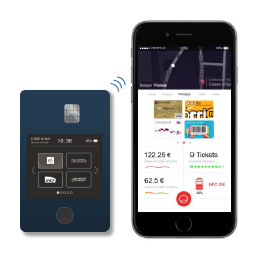
\includegraphics[scale=0.5]{img/carte.png}
			\caption{\label{Carte} Concept de la carte universelle connectée.}			
\end{figure}

Le travail qui nous a été demandé concernait surtout l'aspect bancaire, et plus particulièrement le transport d'informations contextuelles au sein d'une transaction EMV. C'est pourquoi la première partie de notre travail a consisté à étudier la spécification EMV "Payment Tokenisation Specification", de manière à nous familiariser avec la Tokenisation.


\section{Introduction à la Tokenisation}
\subsection{Définition d'un Token}
Dans le cadre d'une transaction, un Token est une donnée "jetable", aussi appelée jeton de paiement, permettant de remplacer les données bancaires telles que le PAN (Personal Account Number).\\
Ainsi, le processus de Tokenisation consiste à générer un Token à partir du PAN et de sa date d'expiration [Figure 1.3].

\begin{figure}[!h]
    \centering
			\includegraphics[scale=0.75]{img/tokeniser2.png}
			\caption{\label{Tokenisation} Principe de la Tokenisation.}			
\end{figure}

Inversement, le processus de Detokenisation permet de récupérer le PAN et sa date d'expiration à partir du Token [Figure 1.4]. 

\begin{figure}[!h]
    \centering
			\includegraphics[scale=0.75]{img/detokeniser.png}
			\caption{\label{Detokenisation} Principe de la Detokenisation.}			
\end{figure}

\subsection{Pourquoi les Token?}
\noindent
\underline{Dans le cadre des transactions EMV}:\\

\noindent
L'utilité des Tokens réside dans le fait qu'ils permettent d'assurer l'intégrité et la confidentialité du PAN lors d'une transaction EMV. En effet, en cas d'interception, le PAN a peu de chance d'être récupéré ce qui limite les risques. Cela permet aux banques émetteurs de réduire la fraude et aux commerçants de ne pas avoir à stocker les informations clients dans leur système d'information.\\

\noindent
De ce fait, les Tokens sont notamment utilisés lors des paiements NFC (Near Field Communication), lors de l'utilisation d'une wallet (i.e. Apple Pay) ou dans le domaine du e-Commerce.\\

\noindent
\underline{Dans le cadre du projet}:\\

\noindent
En plus d'être un élément de sécurité, l'utilisation des Tokens nous permet de transporter de l'information supplémentaire lors des transactions.


\newpage
\section{Planning}
\begin{figure}[!ht]
    \centering
			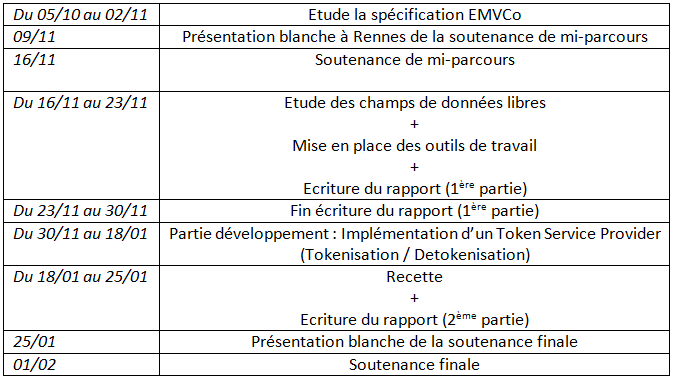
\includegraphics[scale=0.9]{img/planningFinal.png}
			\caption{\label{Planning} Planning final du projet.}			
\end{figure}



\chapter{Etude de la spécification EMVCo "Payment Tokenisation Specification", 2014}
Dans ce chapitre, nous allons revenir sur notre étude de la spécification pour détailler les différentes phases d'une transaction avec Token de façon claire. Dans un premier temps, nous introduirons deux nouveaux acteurs qui n'interviennent pas dans une transaction EMV classique, mais seulement dans une transaction avec Token. Ensuite, nous présenterons les différents éléments de données avant de nous intéresser de plus près à une transaction EMV avec Token, à travers quatre cas d'usage bien précis.\\

\noindent
Ci-dessous se trouve le schéma global d'une transaction EMV avec Token [Figure 2.1]. Dans les parties 2.3, 2.4 et 2.5, nous allons découper ce schéma pour le détailler plus amplement.

\begin{figure}[!ht]
    \centering
			\includegraphics[scale=0.6]{img/TransactionSchemeTokenPAN.png}
			\caption{\label{TransactionScheme} Schéma global d'une transaction EMV avec Token.}			
\end{figure}

 
\section{Token Service Provider et Token Requestor}
\subsection{Token Service Provider}
Le Token Service Provider a pour rôle de fournir les Tokens et de gérer leur cycle de vie. Pour cela, il se doit également d'implémenter toutes les interfaces liées aux services du Token et de garantir la sécurité du Token ainsi que l'association PAN / Token.\\
Lors d'une transaction, le Token Service Provider peut être n'importe quel acteur, c'est-à-dire, la banque émetteur, la banque acquéreur, le commerçant, le réseau de paiement ou encore une tierce partie.

\subsection{Token Requestor}
Le Token Requestor est, quant à lui, responsable des demandes de génération de Token et de changement d'état du Token, notamment en cas de perte ou de vol de celui-ci. Toutefois, avant de pouvoir faire une demande de génération de Token, le Token Requestor doit impérativement s'être au préalable enregistré auprès d'un ou plusieurs Token Service Provider.\\
Lors d'une transaction, le token Requestor peut être la banque émetteur, la banque acquéreur, le commerçant ou bien une tierce partie comme par exemple un gestionnaire de wallet. Cependant, contrairement au Token Service Provider, le Token Requestor ne sera en aucun cas le réseau de paiement.


\section{Les Data elements}
Les Data elements ou éléments de données qui sont utilisés dans une transaction initiée avec un Token, sont présentés dans le schéma ci-dessous [Figure 2.2]. Ils peuvent être obligatoires, conditionnels ou optionnels suivant le message auquel ils appartiennent et suivant l'API utilisée. Tous les réseaux de paiement doivent supporter ces éléments de données lors d'une transaction, pour assurer l'interopérabilité entre les réseaux de paiement.\\

\noindent
Dans un soucis de clarté du schéma, nous avons seulement représenté les éléments de données qui transitent entre deux entités.\\
Pour plus de précisions sur ces éléments de données, consulter la partie 4 de la spécification, "Payment Token Specification Data Elements", à l'adresse suivante: \textit{https://www.emvco.com/specifications.aspx?id=263}.

\begin{figure}[!ht]
    \centering
			\includegraphics[scale=0.5]{img/data_elements.png}
			\caption{\label{DataElements} Eléments de données fournis par une entité à une autre pour une transaction avec Token.}			
\end{figure}

Le Token Vault est un endroit, appartenant au Token Service Provider, dans lequel sont stockés l'association PAN/Token, le Token Requestor ID ainsi que la date d'expiration du Token.


\section{Demande et émission de Token}
Lors d'une transaction EMV, lorsque le PAN n'est pas déjà lié à un Token valide et qu'un Token est requis, le Token Requestor envoie une demande de génération de Token au Token Service Provider. Cette requête contient donc le PAN et sa date d'expiration, ainsi que le Token Requestor ID. Ensuite, le Token service Provider va se charger d'envoyer une demande d'identification et vérification à la banque émetteur, pour déterminer le Token Assurance Level et le Token Assurance Data. Une fois cette étape validée, le Token Service Provider génère le Token qu'il transmet au Token Requestor, en plus de la date d'expiration du Token, du Token Assurance Level et du Token Assurance Data.\\

\noindent
Le schéma suivant résume la demande et l'émission d'un Token [Figure 2.3].

\begin{figure}[!ht]
    \centering
			\includegraphics[scale=0.6]{img/demandeETemissionToken.png}
			\caption{\label{DemandeEmissionToken} Demande et émission d'un Token.}			
\end{figure}

Dans les deux sous-parties qui suivent, nous présenterons davantage les méthodes d'identification et vérification, et les interfaces qui doivent être implémentées par le Token Service Provider.

\subsection{Les méthodes d'Identification et Vérification}

\subsubsection{Généralités}
Les méthodes d'Identification et de Vérification (ID \& V) fournissent la confiance nécessaire à une association entre le PAN et un Token par des vérification diverses sur le porteur ou sur le compte du porteur. Tout cela pour fournir un cadre fiable de paiment par Token. \\
Le Token Assurance Level est une donnée importante pour les paiements utilisant des tokens. Ce Token Assurance Level est dérivé de la méthode d'ID \& V utilisée.
Deux Data Elements sont utilisés pour fournir des informations sur le Token Assurance Level et les méthodes d'ID \& V utilisées.\\
Ce sont les champs : 
\begin{itemize}
	\item Token Assurance Level
	\item Token Assurance Data\\
\end{itemize}

Le Token Service Provider \textbf{DOIT} mettre en place les interfaces nécessaires pour fournir ces deux Data Elements.
Le Token Assurance Level est un nombre compris entre 00 et 99 en fonction du niveau des vérifications effectuées. Le Token Service Provider \textbf{DOIT} également associer le bon Token Assurance Level en fonction des vérifications effectuées.

\subsubsection{Les différentes méthodes}
Il n'y a pas vraiment de méthodes d'ID \& V imposées, mais le Token Service Provider \textbf{DOIT} implémenter une ou plusieurs méthodes d'ID \& V et \textbf{DOIT} assurer que la méthode requise est employé lors de la génération d'un Token. Certaines étapes de ces vérification peuvent être faites par le Token Service Provider, le Token Requestor ou par une tierce partie. Mais dans le cas où les vérifications ne sont pas effectuées par le Token Service Provider, l'entité ayant effectuée une étape de la vérification \textbf{DOIT} fournir des preuves vérifiables du résultat des vérifications.\\
Les vérifications mentionnées dans la spécification sont les suivantes:
\begin{itemize}
	\item Pas de vérification
	\item Vérification du compte (Autorisation à 0 ou autres méthodes.)
	\item Calcul d'un score de risque en utilisant les données du Token Service Provider.
	\item Calcul d'un score de risque en utilisant en plus des données du réseau de paiement.
	\item Vérification du porteur (3DSecure par exemple)
\end{itemize}


\subsection{Les interfaces: Token Service Provider APIs}
\subsubsection{Généralités}
Le Token Service provider \textbf{DOIT} mettre en place une manière sécurisée d'intéragir avec les entités utilisant ses services, à travers par exemple, un Web Service, la norme ISO 8583 ou encore des batches.\\
Le Token Service Provider \textbf{PEUT} implémenter les différentes interfaces et les rendre accessibles aux entités voulant utiliser ses services. Les différentes catégories d'interface sont:
\begin{itemize}
	\item Token Request et Token Assurance
	\item Token Assurance (ID \& V)
	\item De-Tokenisation
	\item Token Routing
	\item Token Lifecycle Management
\end{itemize}
\noindent
Le Token Service Provider \textbf{DOIT} mettre en place au moins une interface par catégorie.

\subsubsection{Token Request et Token Assurance}
Le Token Service Provider \textbf{DOIT} fournir une méthode permettant, à un Token Requestor qui s'est enregistré auprès de lui, de demander l'émission d'un Token.
Le Token Service Provider \textbf{DOIT} aussi mettre en place les contrôles nécessaires pour générer le Token. De plus, il peut effectuer des opérations d'assurance supplémentaires. Dans ce cas, il \textbf{PEUT} indiquer dans sa réponse les mécanismes de vérifications utilisés. 

\subsubsection{Token Assurance}
Toutes ces méthodes sont utilisées si, après l'émission d'un Token, le Token Requestor souhaite faire une mise-à-jour du niveau d'assurance.

\subsubsection{De-Tokenisation}
Le Token Service Provider \textbf{DOIT} mettre en place les contrôles appropriés pour authentifier l'entité qui fait la demande de dé-tokenisation.

\subsubsection{De-Tokenisation avec vérification}
Le Token Service Provider doit, en plus de la dé-tokenisation classique, effectuer des vérifications complémentaires pour s'assurer que le Token est bien utilisé dans un des domaines pour lesquels il a été généré. L'ensemble de ces domaines s'appelle le Token Domain Restriction Controls. 

\subsubsection{Token Lifecycle Management}
Le Token Service Provider \textbf{DOIT} mettre en place des moyens de gérer le cycle de vie d'un Token émis. Ces interfaces peuvent êtres utilisées par de nombreuses entités telles que le réseau de paiement, le Token Requestor, la banque émettrice, etc.\\

\noindent
L'implémentation de TOUTES ces interfaces est laissée à la discretion du Token Service Provider.


\section{Transaction EMV avec Token}
Dans cette section, nous allons d'abord présenter l'interaction client-commerçant de manière à introduire les différents cas d'usage, impliquant un Token, utilisés dans la spécification. Dans un second temps, nous verrons comment se poursuit la transaction avec le Token, depuis le commerçant vers les autres acteurs de la transaction.

\subsection{Côté client - commerçant}
Dans la spécification, l'interaction client - commerçant, lors d'une transaction EMV avec Token, est présentée à travers les paiements NFC mobile, par QR code, par wallet et via les sites de e-Commerce.\\

\noindent
Ce dernier cas est d'ailleurs un peu particulier puisque, lorsque le client fait des achats sur le site d'un commerçant pour la première fois, celui-ci va lui demander de lui envoyer le PAN [Figure 2.4]. En général, le client doit remplir un formulaire avec les données inscrites sur sa carte. Le PAN ne sera pas stocké par le commerçant mais celui-ci va directement contacter le Token Requestor pour qu'il fasse une demande de génération de Token. Par la suite, c'est le Token qui sera stocké par le commerçant. C'est ce qu'on appelle le Card-on-File. Ainsi, le client est en quelque sorte enregistré auprès du commerçant, et lorsqu'il fera d'autres achats sur ce site, le commerçant utilisera le Token lié au PAN du client, qu'il aura conservé dans un fichier. Ici, c'est donc côté commerçant qu'est stocké le Token.\\

\begin{figure}[!ht]
    \centering
			\includegraphics[scale=0.6]{img/cof.png}
			\caption{\label{CardOnFile} Interaction client-commerçant pour le cas d'usage Card-on-file.}			
\end{figure}

Pour les trois autres cas d'usage, le Token est conservé côté client, c'est-à-dire, stocké dans l'appareil du client, qui est son téléphone mobile dans la plupart des cas. En effet, lors d'une transaction, c'est le client qui envoie au commerçant le Token, sa date d'expiration, le Token cryptogram et éventuellement le Token Requestor ID [Figure 2.5].\\
A noter également que, dans le cas du QR code, le client transmet aussi les données du QR code au commerçant. Dans le cas du NFC mobile, il peut y avoir des échanges de données avec un cloud au préalable.

\begin{figure}[!ht]
    \centering
			\includegraphics[scale=0.6]{img/interaction_client-commercant2.png}
			\caption{\label{ClientCommerçant} Interaction client-commerçant pour les cas d'usage: NFC mobile, Wallet, QR Code.}			
\end{figure}

\subsection{Côté commerçant - autres acteurs de la transaction}
Une fois la transaction engagée entre le client et le commerçant, ce dernier envoie une demande d'autorisation à sa banque acquéreur et lui transmet les données que le client lui a envoyé ainsi que le Point Of Sell Entry Mode ou mode d'acceptation [Figure 2.6]. Dans le cas du e-Commerce, l'identifiant du commerçant est également transmis à la banque acquéreur.\\
Ensuite, celle-ci va rediriger toutes ces données vers le réseau de paiement, qui va alors contacter le Token Service Provider pour que celui-ci fasse l'association entre le Token et le PAN correspondant. Le Token Service Provider renvoie donc le PAN au réseau de paiement, mais aussi le Token Assurance Data et le Token Assurance Level. C'est la phase de detokenisation. Ainsi, le réseau de paiement va envoyer les données qu'il a reçu de la banque acquéreur et du Token Service Provider à la banque émetteur, c'est-à-dire, le couple PAN/Token et les données correspondantes. La banque émetteur reçoit donc la demande d'autorisation et peut ou non la valider.\\
Enfin, le résultat de la demande d'autorisation et le PAN sont retransmis au réseau de paiement qui va remplacer le PAN par le Token correspondant, avant de faire recirculer ces données vers la banque acquéreur, qui va les transmettre au commerçant.\\

\noindent
Le schéma ci-dessous résume le déroulement d'une transaction EMV avec Token, à partir du commerçant.

\begin{figure}[!ht]
    \centering
			\includegraphics[scale=0.6]{img/interaction_commercant-autres.png}
			\caption{\label{CommerçantAutresActeurs} Interaction commerçant-autres acteurs de la transaction.}			
\end{figure}


\section{Acquisition, compensation, règlement}
Dans cette partie, nous allons présenter les processus d'acquisition, de compensation et de règlement, qui se déroulent pendant et après la télécollecte.\\

\noindent
Dans le cadre du projet, nous ne nous intéresserons pas à ces trois phases, mais il est nécessaire de les détailler ici puisqu'elles sont présentées dans la spécification.

\subsection{Acquisition et compensation}
Lors de la phase d'acquisition/compensation, le commerçant envoie d'abord un fichier d'acquisition à sa banque acquéreur. Ce fichier contient le Token, sa date d'expiration, le Token Assurance Level et éventuellement le Token Requestor ID. Ensuite, la banque acquéreur vérifie les éléments de données contenus dans ce fichier et y ajoute le mode d'acceptation pour constituer un fichier de compensation qu'elle va envoyer au réseau de paiement. Tout comme pour la transaction, celui-ci va demander au Token Service Provider de faire le mapping entre le Token et le PAN pour pouvoir ensuite transmettre le fichier de compensation complété à la banque émetteur, qui devra valider ou non la compensation et renvoyer sa réponse au réseau de paiement.\\

\newpage
\noindent
Le schéma ci-dessous détaille les champs de données qui transitent lors des phases d'acquisition puis de compensation [Figure 2.7].

\begin{figure}[!ht]
    \centering
			\includegraphics[scale=0.6]{img/CaptureClearing.png}
			\caption{\label{CaptureClearing} Acquisition et compensation d'une transaction réalisée avec un Token.}			
\end{figure}

\subsection{Règlement}
Après avoir validé la transaction et s'être assurée qu'elle avait bien les droits de règlement appropriés, la banque émetteur fournit le PAN, le Token et éventuellement le Token Requestor ID au réseau de paiement. Celui-ci envoie alors le PAN au Token Service Provider qui va effectuer un certain nombre de vérifications sur le Token et sur le mapping PAN/Token, comme par example, s'assurer de la validité du Token ou de l'association avec le PAN. Ensuite, le réseau de paiement transmet le rapport de règlement, contenant le Token, à la banque acquéreur qui le validera ou non.\\

\noindent
Le schéma qui suit représente la phase de règlement vue précédement [Figure 2.8].

\begin{figure}[!ht]
    \centering
			\includegraphics[scale=0.6]{img/Chargeback.png}
			\caption{\label{Reglement} Phase de règlement effectuée après une transaction avec Token.}			
\end{figure}

\end{document}